\documentclass{article}
\usepackage[utf8]{inputenc}
\usepackage{geometry}
\usepackage{tikz}
\usepackage{enumitem}
\usepackage{tabularx}
\usetikzlibrary{shapes,arrows,positioning,calc}

\geometry{a4paper, margin=1in}

\title{\textbf{Assignment 1: Project Proposal}}
\author{Intro to AI Group Project}
\date{\today}

\begin{document}

\maketitle

\section*{Group Members and Expertise}

\begin{enumerate}[label=\textbf{Member \arabic*:}, leftmargin=2cm]
    \item \textbf{Maira Aijaz} (Language \& Content Lead) \\
    \textbf{Expertise:} Arabic vocabulary, word meanings, and basic sentence construction. \\
    \textbf{Role:} Identify core Arabic components (vocabulary, patterns) and define difficulty levels.

    \item \textbf{Muhammad Asad Piracha} (Learning Design \& Dependency Analysis) \\
    \textbf{Expertise:} Language learning methodology and curriculum structuring. \\
    \textbf{Role:} Analyze dependencies between components and design the progression graph.

    \item \textbf{Qadrain Qadri Khan} (AI Tools \& Interaction Design) \\
    \textbf{Expertise:} Use of LLMs and AI-based educational tools. \\
    \textbf{Role:} Explore LLM support for conversation, design AI features (feedback/scoring), and maintain response logs.
\end{enumerate}

\section{Brief Statement of the Problem}
Students of Arabic—particularly those in traditional systems—often struggle with the transition from prescriptive grammar (Sarf and Nahw) to actual language comprehension and usage. As noted in the provided sample research, the abstract and prescriptive nature of these subjects leads to a high cognitive load. This often results in a "bottleneck" where students memorize rules but cannot apply them in real-time conversation, leading to demotivation and high dropout rates. There is a clear need for a tool that bridges this gap by providing low-stakes, interactive practice that reinforces these rules through natural engagement.

\section{Introduction (Motivation \& Project Goal)}
Our project, \textbf{ARABOT}, aims to address the aforementioned problem by acting as an intelligent, conversational practice partner. Unlike traditional dictionaries or static grammar apps, this LLM-powered tool facilitates real-life Arabic conversations tailored to the student’s level.

\textbf{Core Features:}
\begin{itemize}
    \item \textbf{Conversational Immersion:} 5-10 minute conversation practice on random topics.
    \item \textbf{Contextual Support:} Students can ask the AI about unfamiliar words mid-conversation, receiving explanations within the sentence’s context.
    \item \textbf{Performance Feedback:} A detailed analysis and score at the end of each session to track improvement.
\end{itemize}

By following the behaviorist principles of habit formation (as mentioned by Ibn-e-Khaldun) but mitigating the "affective filter" (Krashen) through a supportive AI environment, we aim to lower the cognitive load and make Arabic fluency more achievable.

\section{The ARABOT Methodology: How it Teaches}
\textbf{ARABOT} functions as more than just a chat interface; it is a structured pedagogical tool designed for real-world fluency. The teaching mechanism follows these steps:

\begin{itemize}
    \item \textbf{Level-Aligned Scenarios:} Generates scenarios (e.g., ordering coffee, discussing a book, or travel) matching the student's proficiency.
    \item \textbf{Real-Time Scaffolding:} Provides root (\textit{asl}) and morphological (\textit{seegah}) explanations on demand.
    \item \textbf{Active Feedback Loop:} Captures errors in syntax (Nahw) or morphology (Sarf) to be presented post-session.
    \item \textbf{Quantified Improvement:} Provides a "Performance Score" based on diversity, accuracy, and flow, making learning gamified and fun.
\end{itemize}

\pagebreak

\section{Subject Dependency Graph}
The following graph illustrates the full curriculum dependency, from foundational linguistic "roots" to advanced literary fluency, emphasizing \textbf{ARABOT} as the necessary conversational bridge.

\begin{center}
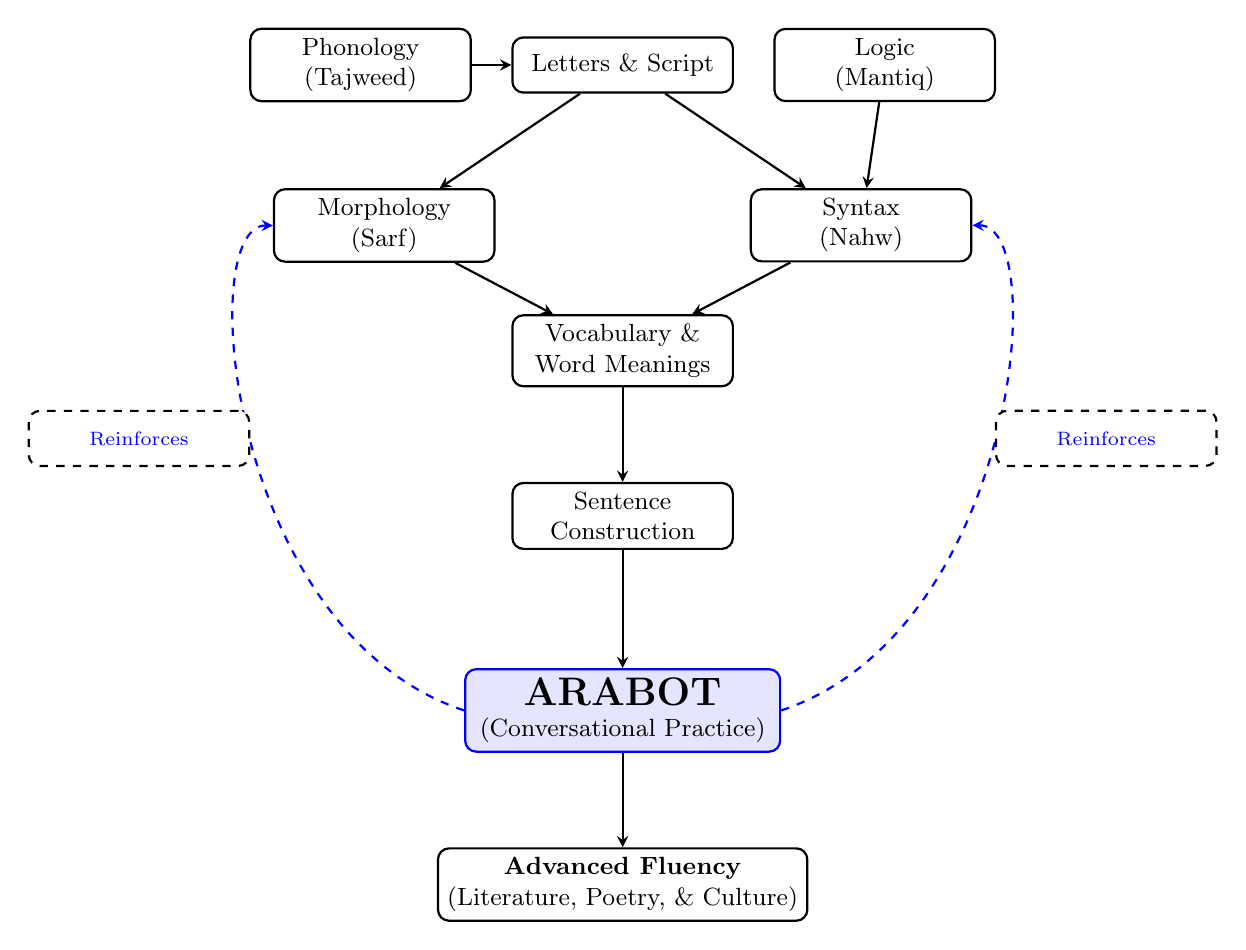
\begin{tikzpicture}[node distance=1.3cm, auto,
    every node/.style={rectangle, draw=black, thick, align=center, rounded corners, fill=white, minimum height=0.7cm, minimum width=2.8cm, font=\small},
    every path/.style={->, >=stealth, thick}
]

    % Foundational Roots (The Basics)
    \node (script) {Letters \& Script};
    \node (phon) [left=0.5cm of script] {Phonology\\(Tajweed)};
    \node (logic) [right=0.5cm of script] {Logic\\(Mantiq)};

    % Core Grammar
    \node (sarf) [below left=1.2cm and 0.2cm of script] {Morphology\\(Sarf)};
    \node (nahw) [below right=1.2cm and 0.2cm of script] {Syntax\\(Nahw)};

    % Progression to Usage
    \node (vocab) [below=2.8cm of script] {Vocabulary \&\\Word Meanings};
    \node (struct) [below=1.2cm of vocab] {Sentence\\Construction};

    % ARABOT (The Project Focus)
    \node (arabot) [below=1.5cm of struct, fill=blue!10, draw=blue, minimum width=4cm] {\Large \textbf{ARABOT}\\(Conversational Practice)};

    % Advanced Level (Simplified & Fun)
    \node (lit) [below=1.2cm of arabot] {\textbf{Advanced Fluency}\\(Literature, Poetry, \& Culture)};

    % Constraints/Edges
    \path (script) edge (sarf) edge (nahw);
    \path (phon) edge (script);
    \path (logic) edge (nahw);
    
    \path (sarf) edge (vocab);
    \path (nahw) edge (vocab);
    \path (vocab) edge (struct);
    \path (struct) edge (arabot);
    
    \path (arabot) edge (lit);
    
    % Feedback
    \draw [->, >=stealth, dashed, blue] (arabot.west) .. controls +(-3,1) and +(-1,0) .. (sarf.west) node [midway, left, font=\scriptsize] {Reinforces};
    \draw [->, >=stealth, dashed, blue] (arabot.east) .. controls +(3,1) and +(1,0) .. (nahw.east) node [midway, right, font=\scriptsize] {Reinforces};

\end{tikzpicture}
\end{center}

\noindent \textbf{Graph Significance:} The graph highlights that while students often learn \textit{Sarf} and \textit{Nahw} as abstract rules, these are dependencies for simple \textit{Sentence Construction}. \textbf{ARABOT} takes these components and turns them into \textit{Conversational Habit}, which is a prerequisite for enjoying advanced material like \textbf{Literature} and \textbf{Poetry}.
\end{document}
